%% §2 — The Hertz Problem  (4 slides)
\section{The Hertz Problem}

%% ── Slide 6: Geometry ───────────────────────────────────────────────────────
\begin{frame}{Hertz Contact: Problem Setup}
\begin{columns}[T]
\begin{column}{0.44\textwidth}
  \centering
  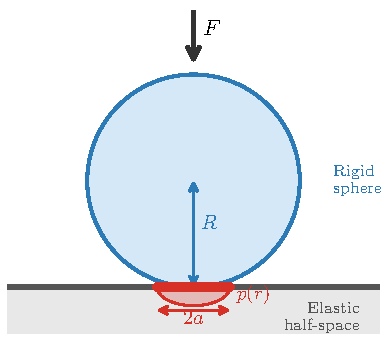
\includegraphics[width=0.88\linewidth]{figures/fig_hertz_geometry.pdf}
\end{column}
\begin{column}{0.52\textwidth}
  \textbf{Rigid sphere} (radius $R$) pressed onto an
  \textbf{elastic half-space} ($\Esta$) with total load $F$.
  \vspace{0.6em}

  Parabolic \textbf{initial gap}:
  \[
    g_0(r) = \frac{r^2}{2R}, \qquad r = \sqrt{x^2+y^2}
  \]
  \textbf{Unknowns}: contact pressure $p(\mathbf{x})$,
  contact radius $a$, approach $\delta$.

  \vspace{0.5em}
  \begin{block}{Boundary conditions in contact ($r<a$)}
    $p \ge 0,\quad u_z = \delta - g_0 \ge 0$
  \end{block}
  \begin{block}{Outside contact ($r\ge a$)}
    $p = 0,\quad u_z < \delta - g_0$
  \end{block}
\end{column}
\end{columns}
\end{frame}

%% ── Slide 7: Analytical solution ────────────────────────────────────────────
\begin{frame}{Hertz Analytical Solution}
\begin{columns}[T]
\begin{column}{0.48\textwidth}
  \textbf{Contact radius}:
  \[
    a = \left(\frac{3FR}{4\Esta}\right)^{1/3}
  \]
  \textbf{Hertzian pressure distribution}:
  \[
    p(r) = p_0\sqrt{1 - \left(\frac{r}{a}\right)^2},
    \quad r \le a
  \]
  \textbf{Peak pressure}:
  \[
    p_0 = \frac{3F}{2\pi a^2}
  \]
  \textbf{Indentation}:
  \[
    \delta = \frac{a^2}{R}
  \]
\end{column}
\begin{column}{0.48\textwidth}
  \begin{tikzpicture}[scale=0.88]
    % Hertz pressure half-arch sketch
    \begin{axis}[
      width=6.5cm, height=4.5cm,
      axis lines=left,
      xlabel={$r/a$}, ylabel={$p/p_0$},
      xmin=0, xmax=1.3, ymin=0, ymax=1.15,
      xtick={0,0.5,1.0},
      ytick={0,0.5,1.0},
      tick label style={font=\small},
      label style={font=\small},
      clip=false,
    ]
    \addplot[domain=0:1, samples=200, thick, mblue]
      {sqrt(max(0,1-x*x))};
    \addplot[domain=1:1.25, samples=5, thick, mblue]
      {0};
    \addplot[only marks, mark=*, mark size=1.8pt, mred]
      coordinates {(0,1)};
    \draw[dashed,mgray] (axis cs:1,0) -- (axis cs:1,0.1);
    \node[font=\small] at (axis cs:1.05,0.07) {$r=a$};
    \node[font=\small,mblue] at (axis cs:0.55,0.7)
      {$\sqrt{1-(r/a)^2}$};
    \end{axis}
  \end{tikzpicture}
\end{column}
\end{columns}
\end{frame}

%% ── Slide 8: BEM discretisation + Polonsky–Keer ─────────────────────────────
\begin{frame}{BEM Discretisation \& Polonsky--Keer Algorithm}
\begin{columns}[T]
\begin{column}{0.50\textwidth}
  Grid $N_s\!\times\!N_s$, element size $h=L/N_s$, flat index $k=i_y N_s+i_x$:
  \[
    S_{ij} = \frac{\calL(\mathbf{x}_i - \mathbf{x}_j,\;h/2)}{\pi\Esta}
  \]
  \vspace{-0.3em}
  \textbf{Contact QP}:
  \[
    \min_{p}\;\tfrac{1}{2}p^\T Sp + p^\T g_0
    \;\text{s.t.}\;p_i\ge0,\;\bar p = p_{\rm nom}
  \]
\end{column}
\begin{column}{0.46\textwidth}
  \begin{block}{Polonsky--Keer (1999) PCG}
    \small
    \begin{enumerate}
      \item Init $p = \pbar\mathbf{1}$; $u = Sp$; $r = u+g_0$
      \item Shift: $\bar r = r - \langle r\rangle_{\rm contact}$
      \item Zero $r_i$ if $p_i=0$ and $\bar r_i \ge 0$
      \item $\delta = \|r\|^2$; \textbf{converge} if $\delta<\varepsilon^2\delta_0$
      \item $t = r + (\delta/\delta_{\rm old})\,t$; mask $t$
      \item $v=St$;\; $\tau = \langle r,t\rangle/\langle v,t\rangle_{\rm c}$
      \item $p \mathrel{-}= \tau t$;\; $p \leftarrow \max(p,0)$
      \item Overlap correction;\; normalise $p$
      \item $u = Sp$;\; $r = u+g_0$
    \end{enumerate}
  \end{block}
\end{column}
\end{columns}
\end{frame}

%% ── Slide 9: Hertz validation ───────────────────────────────────────────────
\begin{frame}{Hertz Validation ($N_s=64$, $\Esta=1$, $R=0.5$)}
  \centering
  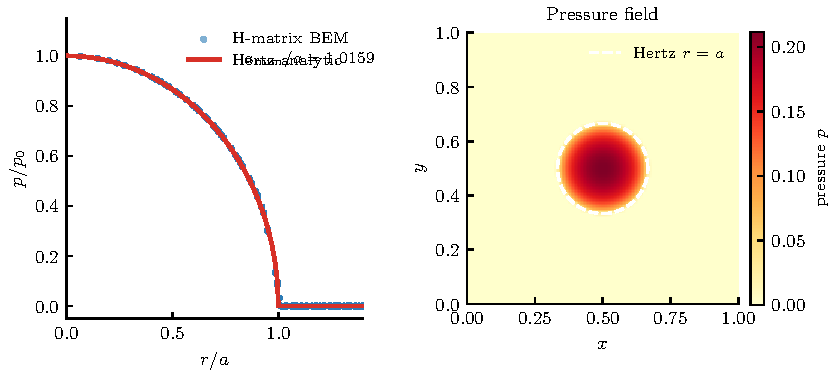
\includegraphics[width=0.92\linewidth]{figures/fig_hertz_validation.pdf}
  \vspace{0.3em}

  \begin{columns}
  \begin{column}{0.48\textwidth}
    \centering
    {\small
    $a_{\rm num}/a_{\rm Hertz} = 1.016$ \quad
    $p_{\rm max}/p_0 = 0.998$
    }
  \end{column}
  \begin{column}{0.48\textwidth}
    \centering
    {\small
    Mean pressure error $< 10^{-10}$\quad
    Converged in 29 iterations
    }
  \end{column}
  \end{columns}
\end{frame}
